\section{奇异同调群}
\sourcepage{187--188}
本节定义奇异同调群，并建立它们的一些初等性质。先引入记号。

以 $\R^\infty$ 表示 $E^J$，其中 $J=\Z_+$ 是正整数集；它的点是只有有限个非零项的实数序列。记 $\epsilon_0=0$，并以 $\epsilon_1,\epsilon_2,\ldots$ 表示通常的基向量。由 $\epsilon_0,\ldots,\epsilon_p$ 张成的单形称为\textbf{标准 $p$ 维单形}（standard $p$-simplex），记作 $\Delta_p$。于是 $\Delta_{p-1}$ 是 $\Delta_p$ 的一个面。

拓扑空间 $X$ 中的一个\textbf{奇异 $p$ 维单形}（singular $p$-simplex）是连续映射 $T:\Delta_p\to X$。这里的映射不必是嵌入，甚至可以是常值映射。以 $S_p(X)$ 表示以所有奇异 $p$ 维单形为基的自由阿贝尔群，称为 $X$ 的 $p$ 维\textbf{奇异链群}（singular chain group）。它的元素称为奇异 $p$ 维链，是奇异单形的有限整数线性组合。

若 $a_0,\ldots,a_p$ 是 $E^J$ 中任意一些点（不要求几何独立），则存在唯一的仿射映射 $\Delta_p\to E^J$，将 $\epsilon_i$ 映至 $a_i$。称它为\textbf{线性奇异单形}（linear singular simplex），记作 $\ell(a_0,\ldots,a_p)$。具体地，
\[
\ell(a_0,\ldots,a_p)(x_1,\ldots,x_p,0,\ldots)
=a_0+\sum_{i=1}^p x_i(a_i-a_0).
\]
\translatornote{原书此处求和上限印为 $n$；按所定义的 $p$ 维单形，应为 $p$。}
特别地，$\ell(\epsilon_0,\ldots,\epsilon_p)$ 是 $\Delta_p$ 到 $\R^\infty$ 的包含映射。而
\[
\ell(\epsilon_0,\ldots,\widehat\epsilon_i,\ldots,\epsilon_p):\Delta_{p-1}\longrightarrow\Delta_p
\]
将 $\Delta_{p-1}$ 线性同胚地映到 $\Delta_p$ 的第 $i$ 个面。将它与 $T$ 复合，所得奇异 $(p-1)$ 维单形称为 $T$ 的第 $i$ 个面。

\sourcepage{189}
定义\textbf{边缘算子} $\partial:S_p(X)\to S_{p-1}(X)$：在基元上令
\[
\partial T=\sum_{i=0}^p(-1)^iT\circ\ell(\epsilon_0,\ldots,\widehat\epsilon_i,\ldots,\epsilon_p),
\]
再线性延拓。\translatornote{原书这一定义中的符号印为 $(-1)^p$；应为随面指标交替的 $(-1)^i$。}若 $f:X\to Y$ 连续，则定义同态 $f_\#:S_p(X)\to S_p(Y)$，使 $f_\#T=f\circ T$。

\entry{定理}{4.2.1}同态 $f_\#$ 与 $\partial$ 可交换，并且 $\partial^2=0$。

\textbf{证明：}对任一奇异单形 $T$，
\begin{align*}
\partial f_\#T&=\sum_{i=0}^p(-1)^i(f\circ T)\circ\ell(\epsilon_0,\ldots,\widehat\epsilon_i,\ldots,\epsilon_p),\\
f_\#\partial T&=\sum_{i=0}^p(-1)^if\circ\bigl(T\circ\ell(\epsilon_0,\ldots,\widehat\epsilon_i,\ldots,\epsilon_p)\bigr).
\end{align*}
两者由复合的结合律相等。对于线性奇异单形，线性映射的复合仍为线性映射，因而
\[
\partial\ell(a_0,\ldots,a_p)=\sum_{i=0}^p(-1)^i\ell(a_0,\ldots,\widehat a_i,\ldots,a_p).
\]
像引理 1.6.9 的证明一样展开两次边缘，每一项出现两次，符号相反，故在线性奇异单形上 $\partial^2=0$。对一般的 $T$，注意
\[
T=T_\#\bigl(\ell(\epsilon_0,\ldots,\epsilon_p)\bigr).
\]
由刚证明的交换性，$\partial^2T=T_\#\partial^2\ell(\epsilon_0,\ldots,\epsilon_p)=0$。\hfill$\square$

\sourcepage{190}
\entry{定义}{4.2.2}群 $S_p(X)$ 连同边缘算子构成的链复形记为 $\mathcal S(X)$，称为 $X$ 的\textbf{奇异链复形}（singular chain complex）。它的同调群称为 $X$ 的\textbf{奇异同调群}（singular homology groups），记为 $H_p(X)$。这一记号与第 3.6 节的单纯同调群相同；第 4.7 节将证明两者之间有自然同构。

定义增广同态 $\epsilon:S_0(X)\to\Z$，将每个奇异零维单形映为 $1$。对于奇异一维单形 $T$，有 $\epsilon\partial T=0$，所以可定义约化奇异同调群 $\widetilde H_p(X)$。映射 $f_\#$ 保持增广，故在普通及约化同调群上都诱导同态 $f_*$。若所有约化奇异同调群都为零，称 $X$ \textbf{无环}。

\entry{定理}{4.2.3}恒等映射诱导恒等同态；若 $f:X\to Y$、$g:Y\to Z$ 连续，则 $(g\circ f)_*=g_*\circ f_*$。这对普通及约化奇异同调均成立。

\textbf{证明：}这些等式在链的层次上已经成立：$i_\#T=T$，且 $(g\circ f)_\#T=g_\#f_\#T$。\hfill$\square$

\entry{推论}{4.2.4}若 $h:X\to Y$ 是同胚，则 $h_*$ 是同构。

因此，奇异同调群的拓扑不变性立刻得到；与第二章中证明单纯同调群拓扑不变性所需的工作相比，这一点十分显著。

\entry{定理}{4.2.5}在 $X$ 的每个道路分支 $X_\alpha$ 中选取一个奇异零维单形 $T_\alpha$。则 $H_0(X)$ 是自由阿贝尔群，以诸 $T_\alpha$ 的同调类为基。群 $\widetilde H_0(X)$ 也是自由阿贝尔群：若 $X$ 道路连通，它为零；否则，固定 $\alpha_0$，则诸 $T_\alpha-T_{\alpha_0}$（$\alpha\ne\alpha_0$）的同调类构成一组基。

\sourcepage{191}
\textbf{证明：}设奇异零维单形 $T$ 的像为点 $x\in X_\alpha$。从 $x$ 到 $T_\alpha(\Delta_0)$ 的一条道路 $f:[0,1]\to X$ 是奇异一维单形，且 $\partial f=T_\alpha-T$。故每个零维链均同调于某个有限和 $\sum n_\alpha T_\alpha$。

若 $\sum n_\alpha T_\alpha=\partial d$，每个奇异一维单形的像道路连通，因而完全包含于某个 $X_\alpha$。可相应写成 $d=\sum d_\alpha$，其中 $d_\alpha\in S_1(X_\alpha)$。比较各道路分支内的基元，得 $n_\alpha T_\alpha=\partial d_\alpha$。施以增广，得 $n_\alpha=0$。这证明了线性无关性。\translatornote{原书在此还说“因此 $d=0$”；这个结论一般不成立，因为 $d$ 可以是非零闭链。实际所需且已经证明的是所有 $n_\alpha=0$。}关于约化同调的结论，用与定理 1.8.3 相同的论证即可得到。\hfill$\square$

下面把星形凸性的概念推广到 $E^J$ 的子空间。

\entry{定义}{4.2.6}若 $w\in X\subset E^J$，且连接 $X$ 中每个点与 $w$ 的线段都包含于 $X$，则称 $X$ \textbf{关于 $w$ 星形凸}（star convex relative to $w$）。

\entry{定义}{4.2.7}设 $X$ 关于 $w$ 星形凸，$T:\Delta_p\to X$ 为奇异单形。定义 $[T,w]:\Delta_{p+1}\to X$：对于 $x\in\Delta_p$，将从 $x$ 到 $\epsilon_{p+1}$ 的线段线性地映到从 $T(x)$ 到 $w$ 的线段。对链 $c=\sum n_iT_i$，令 $[c,w]=\sum n_i[T_i,w]$。这与第 1.9 节的括号运算类似，不过顶点现在写在末尾。

映射 $[T,w]$ 在 $\Delta_p$ 上的限制为 $T$。若 $T=\ell(a_0,\ldots,a_p)$，则 $[T,w]=\ell(a_0,\ldots,a_p,w)$。

为证明连续性，考虑商映射
\[
\pi:\Delta_p\times I\to\Delta_{p+1},\qquad \pi(x,t)=(1-t)x+t\epsilon_{p+1},
\]
它把 $\Delta_p\times\{1\}$ 压缩为一点。连续映射 $f(x,t)=(1-t)T(x)+tw$ 在该集合上为常值，故通过 $\pi$ 诱导一个从 $\Delta_{p+1}$ 到 $X$ 的连续映射。\translatornote{原书将此处的常值集合写为 $\Delta_p$；应为 $\Delta_p\times\{1\}$。}

\sourcepage{192}
\begin{center}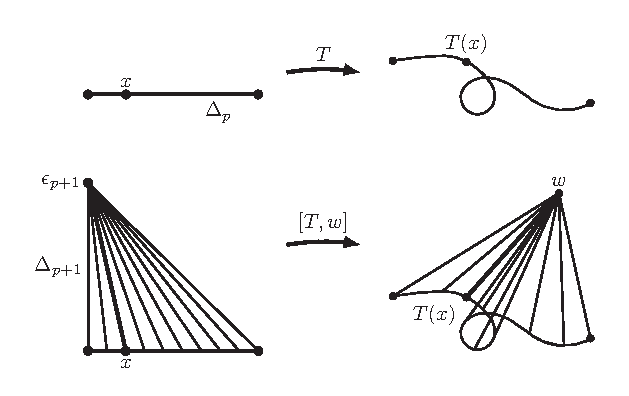
\includegraphics[width=.87\textwidth]{figures/4-2-1.pdf}\\图 4.2.1\end{center}
由于 $\pi$ 将 $\{x\}\times I$ 线性地映到从 $x$ 到 $\epsilon_{p+1}$ 的线段，而 $f$ 将它线性地映到从 $T(x)$ 到 $w$ 的线段，这个诱导映射恰好是 $[T,w]$。因此 $[T,w]$ 连续。现在计算括号运算与边缘算子的关系。

\entry{引理}{4.2.8}设 $X$ 关于 $w$ 星形凸，$c$ 是 $X$ 中的奇异 $p$ 维链，则
\[
\partial[c,w]=\begin{cases}[\partial c,w]+(-1)^{p+1}c,&p>0,\\\epsilon(c)T_w-c,&p=0,\end{cases}
\]
其中 $T_w$ 是将 $\Delta_0$ 映到 $w$ 的奇异零维单形。

\textbf{证明：}若 $T$ 为零维单形，则 $[T,w]$ 将 $\Delta_1$ 线性地映到从 $T(\Delta_0)$ 到 $w$ 的线段，所以 $\partial[T,w]=T_w-T$。由线性性得第二个公式。

设 $p>0$。只需对奇异 $p$ 维单形 $T$ 验证第一个公式。图 4.2.2 说明了 $p=1$ 的情形。由定义，
\[
\partial[T,w]=\sum_{i=0}^{p+1}(-1)^i[T,w]\circ\ell(\epsilon_0,\ldots,\widehat\epsilon_i,\ldots,\epsilon_{p+1}).\tag{*}
\]
\sourcepage{193}
简记 $\ell_i=\ell(\epsilon_0,\ldots,\widehat\epsilon_i,\ldots,\epsilon_{p+1})$。
\begin{center}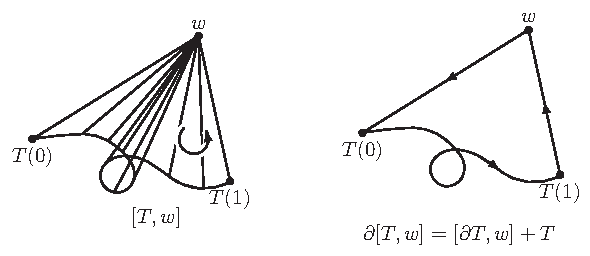
\includegraphics[width=.85\textwidth]{figures/4-2-2.pdf}\\图 4.2.2\end{center}
映射 $\ell_{p+1}$ 是 $\Delta_p$ 到 $\Delta_{p+1}$ 的包含映射，而 $[T,w]|_{\Delta_p}=T$，故式 (*) 的末项为 $(-1)^{p+1}T$。

再考虑 $i<p+1$。映射 $\ell_i$ 将 $\Delta_p$ 线性同胚地映到 $\Delta_{p+1}$ 的第 $i$ 个面，并将顶点 $\epsilon_0,\ldots,\epsilon_p$ 依次映到 $\epsilon_0,\ldots,\widehat\epsilon_i,\ldots,\epsilon_{p+1}$。所以其在 $\Delta_{p-1}$ 上的限制满足
\[
\ell_i|_{\Delta_{p-1}}=\ell(\epsilon_0,\ldots,\widehat\epsilon_i,\ldots,\epsilon_p).\tag{**}
\]
对于 $x\in\Delta_{p-1}$，$\ell_i$ 将从 $x$ 到 $\epsilon_p$ 的线段线性地映到从 $\ell_i(x)$ 到 $\epsilon_{p+1}$ 的线段。因为 $\ell_i(x)\in\Delta_p$，$[T,w]$ 又将后一线段线性地映到从 $T(\ell_i(x))$ 到 $w$ 的线段。因此，
\[
[T,w]\circ\ell_i=[T\circ(\ell_i|_{\Delta_{p-1}}),w].
\]
\translatornote{原书此等式左端漏印了复合映射 $\circ\ell_i$。}代入 (*) 并使用 (**)，得
\begin{align*}
\partial[T,w]&=\sum_{i=0}^{p}(-1)^i[T\circ\ell(\epsilon_0,\ldots,\widehat\epsilon_i,\ldots,\epsilon_p),w]+(-1)^{p+1}T\\
&=[\partial T,w]+(-1)^{p+1}T.
\end{align*}
\hfill$\square$

\entry{定理}{4.2.9}若 $X\subset E^J$ 关于 $w$ 星形凸，则 $X$ 的奇异同调无环。

\sourcepage{194}
\textbf{证明：}若零维链 $c$ 满足 $\epsilon(c)=0$，则上述引理给出 $\partial[c,w]=\epsilon(c)T_w-c=-c$，故 $c$ 是边缘，$\widetilde H_0(X)=0$。若 $z$ 是 $p>0$ 维闭链，则
\[
\partial[z,w]=[\partial z,w]+(-1)^{p+1}z=(-1)^{p+1}z,
\]
故 $z$ 也是边缘，$H_p(X)=0$。\hfill$\square$

\entry{推论}{4.2.10}任意单形的奇异同调无环。

\entry{定义}{4.2.11}图 4.2.3 中的\textbf{拓扑学家的正弦曲线}（topologist's sine curve）是 $\R^2$ 的子空间
\[
Y=\{(x,\sin(1/x)):0<x\le1\}\cup\{(0,y):-1\le y\le1\}.
\]
习题 1(b) 将用到这个空间。
\begin{center}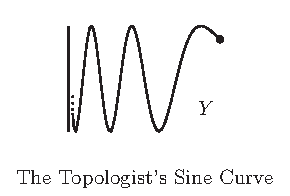
\includegraphics[width=.48\textwidth]{figures/4-2-3.pdf}\\图 4.2.3：拓扑学家的正弦曲线\end{center}

\subsection*{习题}
\begin{enumerate}
\item \begin{enumerate}[label=(\alph*)]
\item 设 $\{X_\alpha\}$ 是 $X$ 的道路分支全体。证明 $H_p(X)\cong\bigoplus_\alpha H_p(X_\alpha)$。
\item 计算拓扑学家的正弦曲线 $Y$ 的奇异同调。
\end{enumerate}
\item 设 $X$ 是 $\R^N$ 的紧子空间，$f:X\to Y$。
\begin{enumerate}[label=(\alph*)]
\item 设 $w=(0,0,\ldots,0,1)\in\R^N\times\R$，$C$ 是连接 $X$ 中各点与 $w$ 的所有线段之并。证明 $C$ 是 $X\times I$ 的商空间。
\item 证明：若 $f$ 同伦于常值映射，则在约化同调中 $f_*$ 是零同态。〔提示：证明 $f$ 可以延拓到 $C$。〕
\item 证明：若 $X$ 可缩，则 $X$ 无环。
\end{enumerate}
\item 计算 $\R^2$ 中单位圆盘的 $H_1$。
\item 证明：若 $U\subset\R^2$ 同胚于单位圆盘，则对每个 $p>0$，都有 $H_p(U)=0$。
\end{enumerate}
